\PassOptionsToPackage{unicode=true}{hyperref} % options for packages loaded elsewhere
\PassOptionsToPackage{hyphens}{url}
%
\documentclass[a4paper,11pt]{memoir}
\usepackage{lmodern}
\usepackage{amssymb,amsmath}
\usepackage{ifxetex,ifluatex}
\usepackage{fixltx2e} % provides \textsubscript
\ifnum 0\ifxetex 1\fi\ifluatex 1\fi=0 % if pdftex
  \usepackage[T1]{fontenc}
  \usepackage[utf8]{inputenc}
  \usepackage{textcomp} % provides euro and other symbols
\else % if luatex or xelatex
  \usepackage{unicode-math}
  \defaultfontfeatures{Ligatures=TeX,Scale=MatchLowercase}
\fi
% use upquote if available, for straight quotes in verbatim environments
\IfFileExists{upquote.sty}{\usepackage{upquote}}{}
% use microtype if available
\IfFileExists{microtype.sty}{%
\usepackage[]{microtype}
\UseMicrotypeSet[protrusion]{basicmath} % disable protrusion for tt fonts
}{}
\IfFileExists{parskip.sty}{%
\usepackage{parskip}
}{% else
\setlength{\parindent}{0pt}
\setlength{\parskip}{6pt plus 2pt minus 1pt}
}
\usepackage{hyperref}
\hypersetup{
            pdftitle={Dates and missing dating data in "sdam"},
            pdfauthor={Antonio Rivero Ostoic},
            pdfborder={0 0 0},
            breaklinks=true}
\urlstyle{same}  % don't use monospace font for urls
\usepackage[left=2cm,right=2cm,top=2cm,bottom=2cm]{geometry}
\usepackage{color}
\usepackage{fancyvrb}
\newcommand{\VerbBar}{|}
\newcommand{\VERB}{\Verb[commandchars=\\\{\}]}
\DefineVerbatimEnvironment{Highlighting}{Verbatim}{commandchars=\\\{\}}
% Add ',fontsize=\small' for more characters per line
\usepackage{framed}
\definecolor{shadecolor}{RGB}{248,248,248}
\newenvironment{Shaded}{\begin{snugshade}}{\end{snugshade}}
\newcommand{\AlertTok}[1]{\textcolor[rgb]{0.94,0.16,0.16}{#1}}
\newcommand{\AnnotationTok}[1]{\textcolor[rgb]{0.56,0.35,0.01}{\textbf{\textit{#1}}}}
\newcommand{\AttributeTok}[1]{\textcolor[rgb]{0.77,0.63,0.00}{#1}}
\newcommand{\BaseNTok}[1]{\textcolor[rgb]{0.00,0.00,0.81}{#1}}
\newcommand{\BuiltInTok}[1]{#1}
\newcommand{\CharTok}[1]{\textcolor[rgb]{0.31,0.60,0.02}{#1}}
\newcommand{\CommentTok}[1]{\textcolor[rgb]{0.56,0.35,0.01}{\textit{#1}}}
\newcommand{\CommentVarTok}[1]{\textcolor[rgb]{0.56,0.35,0.01}{\textbf{\textit{#1}}}}
\newcommand{\ConstantTok}[1]{\textcolor[rgb]{0.00,0.00,0.00}{#1}}
\newcommand{\ControlFlowTok}[1]{\textcolor[rgb]{0.13,0.29,0.53}{\textbf{#1}}}
\newcommand{\DataTypeTok}[1]{\textcolor[rgb]{0.13,0.29,0.53}{#1}}
\newcommand{\DecValTok}[1]{\textcolor[rgb]{0.00,0.00,0.81}{#1}}
\newcommand{\DocumentationTok}[1]{\textcolor[rgb]{0.56,0.35,0.01}{\textbf{\textit{#1}}}}
\newcommand{\ErrorTok}[1]{\textcolor[rgb]{0.64,0.00,0.00}{\textbf{#1}}}
\newcommand{\ExtensionTok}[1]{#1}
\newcommand{\FloatTok}[1]{\textcolor[rgb]{0.00,0.00,0.81}{#1}}
\newcommand{\FunctionTok}[1]{\textcolor[rgb]{0.00,0.00,0.00}{#1}}
\newcommand{\ImportTok}[1]{#1}
\newcommand{\InformationTok}[1]{\textcolor[rgb]{0.56,0.35,0.01}{\textbf{\textit{#1}}}}
\newcommand{\KeywordTok}[1]{\textcolor[rgb]{0.13,0.29,0.53}{\textbf{#1}}}
\newcommand{\NormalTok}[1]{#1}
\newcommand{\OperatorTok}[1]{\textcolor[rgb]{0.81,0.36,0.00}{\textbf{#1}}}
\newcommand{\OtherTok}[1]{\textcolor[rgb]{0.56,0.35,0.01}{#1}}
\newcommand{\PreprocessorTok}[1]{\textcolor[rgb]{0.56,0.35,0.01}{\textit{#1}}}
\newcommand{\RegionMarkerTok}[1]{#1}
\newcommand{\SpecialCharTok}[1]{\textcolor[rgb]{0.00,0.00,0.00}{#1}}
\newcommand{\SpecialStringTok}[1]{\textcolor[rgb]{0.31,0.60,0.02}{#1}}
\newcommand{\StringTok}[1]{\textcolor[rgb]{0.31,0.60,0.02}{#1}}
\newcommand{\VariableTok}[1]{\textcolor[rgb]{0.00,0.00,0.00}{#1}}
\newcommand{\VerbatimStringTok}[1]{\textcolor[rgb]{0.31,0.60,0.02}{#1}}
\newcommand{\WarningTok}[1]{\textcolor[rgb]{0.56,0.35,0.01}{\textbf{\textit{#1}}}}
\usepackage{graphicx,grffile}
\makeatletter
\def\maxwidth{\ifdim\Gin@nat@width>\linewidth\linewidth\else\Gin@nat@width\fi}
\def\maxheight{\ifdim\Gin@nat@height>\textheight\textheight\else\Gin@nat@height\fi}
\makeatother
% Scale images if necessary, so that they will not overflow the page
% margins by default, and it is still possible to overwrite the defaults
% using explicit options in \includegraphics[width, height, ...]{}
\setkeys{Gin}{width=\maxwidth,height=\maxheight,keepaspectratio}
\setlength{\emergencystretch}{3em}  % prevent overfull lines
\providecommand{\tightlist}{%
  \setlength{\itemsep}{0pt}\setlength{\parskip}{0pt}}
\setcounter{secnumdepth}{0}
% Redefines (sub)paragraphs to behave more like sections
\ifx\paragraph\undefined\else
\let\oldparagraph\paragraph
\renewcommand{\paragraph}[1]{\oldparagraph{#1}\mbox{}}
\fi
\ifx\subparagraph\undefined\else
\let\oldsubparagraph\subparagraph
\renewcommand{\subparagraph}[1]{\oldsubparagraph{#1}\mbox{}}
\fi

% set default figure placement to htbp
\makeatletter
\def\fps@figure{htbp}
\makeatother

\usepackage{hyperref}
\PassOptionsToPackage{bookmarks=false}{hyperref}

\makeatletter 
\renewcommand{\figurename}{Fig.}
\renewcommand{\thefigure}{\@arabic\c@figure}
\makeatother

\setcounter{page}{15}
\setcounter{figure}{3}

\title{Dates and missing dating data in \texttt{"sdam"}}
\author{Antonio Rivero Ostoic}
\date{September 2022}

\begin{document}
\maketitle

%   \hypertarget{preliminaries}{%
%   \subsection{Preliminaries}\label{preliminaries}}
%   
%   Install and load a version of \texttt{"sdam"} package.
%   
%   \begin{Shaded}
%   \begin{Highlighting}[]
%   \KeywordTok{install.packages}\NormalTok{(}\StringTok{"sdam"}\NormalTok{) }\CommentTok{# from CRAN}
%   \NormalTok{devtools}\OperatorTok{::}\KeywordTok{install_github}\NormalTok{(}\StringTok{"sdam-au/sdam"}\NormalTok{) }\CommentTok{# development version}
%   \NormalTok{devtools}\OperatorTok{::}\KeywordTok{install_github}\NormalTok{(}\StringTok{"mplex/cedhar"}\NormalTok{, }\DataTypeTok{subdir=}\StringTok{"pkg/sdam"}\NormalTok{) }\CommentTok{# legacy version R 3.6.x}
%   \end{Highlighting}
%   \end{Shaded}

\begin{Shaded}
\begin{Highlighting}[]
\CommentTok{# load and check versions}
\KeywordTok{library}\NormalTok{(sdam)}
\KeywordTok{packageVersion}\NormalTok{(}\StringTok{"sdam"}\NormalTok{)}
\end{Highlighting}
\end{Shaded}

\begin{verbatim}
[1] '1.0.0'
\end{verbatim}

\hypertarget{dating-data}{%
\section{Dating data}\label{dating-data}}

Temporal data is significant when it comes to analysing the history of
archaeological artefacts like written markers from the Ancient
Mediterranean. In the \texttt{EDH} dataset, for example, dates for
inscriptions are plausible timespans of existence with the endpoints in
variables \texttt{not\_before} and \texttt{not\_after} that, from the
perspective of the timespan, are the \emph{terminus ante quem} (TAQ) and
\emph{terminus post quem} (TPQ) of the time segment. However, not all
inscriptions have these two variables filled by domain experts and
replacing missing dating data constitutes a challenge.

Besides \texttt{EDH}, other datasets with \texttt{"sdam"} the package
and related functions involve dating data in the ancient Mediterranean
like displaying dates and time segments in a plot, by organising dates
within Roman provinces, and by performed imputation techniques for
missing dating data.

\hypertarget{plotting-temporal-data}{%
\subsection{Plotting temporal data}\label{plotting-temporal-data}}

\hypertarget{shipwrecks-dataset-dating-data}{%
\subsubsection{Shipwrecks dataset dating
data}\label{shipwrecks-dataset-dating-data}}

An example of plotting dates is with the Shipwrecks external dataset,
which is a semicolon separated file of different variables.

References for shipwrecks data are in

\begin{itemize}
\tightlist
\item
  Vignette \href{../doc/Intro.html}{Datasets in \texttt{"sdam"} package}
\end{itemize}

When reading the shipwrecks external dataset with \texttt{read.csv} make
sure to use the right separator in \texttt{sep} and leave untouched the
names of the variables.

\begin{Shaded}
\begin{Highlighting}[]
\CommentTok{# load shipwrecks external dataset}
\NormalTok{sw <-}\StringTok{ }\KeywordTok{system.file}\NormalTok{(}\StringTok{"extdata"}\NormalTok{,}\StringTok{"StraussShipwrecks.csv"}\NormalTok{,}\DataTypeTok{package=}\StringTok{"sdam"}\NormalTok{) }\OperatorTok{|}\ErrorTok{>}\StringTok{ }
\StringTok{  }\KeywordTok{read.csv}\NormalTok{(}\DataTypeTok{sep=}\StringTok{";"}\NormalTok{, }\DataTypeTok{check.names=}\OtherTok{FALSE}\NormalTok{)}
\end{Highlighting}
\end{Shaded}

\begin{Shaded}
\begin{Highlighting}[]
\CommentTok{# variables in shipwrecks dataset}
\KeywordTok{colnames}\NormalTok{(sw)}
\end{Highlighting}
\end{Shaded}

\begin{verbatim}
 [1] "Wreck ID"                "Strauss ID"              "Name"                   
 [4] "Parker Number"           "Sea area"                "Country"                
 [7] "Region"                  "Latitude"                "Longitude"              
[10] "Min depth"               "Max depth"               "Depth"                  
[13] "Period"                  "Dating"                  "Earliest date"          
[16] "Latest date"             "Date range"              "Mid point of date range"
[19] "Probability"             "Place of origin"         "Place of destination"   
[22] "Reference"               "Comments"                "Amphorae"               
[25] "Marble"                  "Columns etc"             "Sarcophagi"             
[28] "Blocks"                  "Marble type"             "Other cargo"            
[31] "Hull remains"            "Shipboard paraphernalia" "Ship equipment"         
[34] "Estimated tonnage"       "Amphora type"           
\end{verbatim}

Plot the time segments with function \texttt{plot.dates()} and a
customized \texttt{\textquotesingle{}id\textquotesingle{}} where
variables 15 to 16 in \texttt{sw} have timespans of existence as
\texttt{\textquotesingle{}taq\textquotesingle{}} and
\texttt{\textquotesingle{}tpq\textquotesingle{}}.

\begin{Shaded}
\begin{Highlighting}[]
\CommentTok{# shipwrecks dates with Wreck ID}
\KeywordTok{plot.dates}\NormalTok{(sw, }\DataTypeTok{id=}\StringTok{"Wreck ID"}\NormalTok{, }\DataTypeTok{type=}\StringTok{"rg"}\NormalTok{, }\DataTypeTok{taq=}\StringTok{"Earliest date"}\NormalTok{, }\DataTypeTok{tpq=}\StringTok{"Latest date"}\NormalTok{, }\DataTypeTok{col=}\DecValTok{4}\NormalTok{)}
\end{Highlighting}
\end{Shaded}

\begin{figure}

\centering
\includegraphics[width=6cm, trim=0 0 0 40, clip]{img/unnamed-chunk-5-1} %lbrt
%{\centering \includegraphics{Dates_files/figure-latex/unnamed-chunk-5-1} 
%}

\caption{Range of timespans in Shipwrecks dataset}\label{fig:unnamed-chunk-5}
\end{figure}

\hypertarget{mid-points-and-range-of-timespan}{%
\subsubsection{Mid points and range of
timespan}\label{mid-points-and-range-of-timespan}}

The mid points and range of shipwrecks data are explicitly computed by
function \texttt{prex()} with the \texttt{mp} option in the
\texttt{\textquotesingle{}type\textquotesingle{}} argument.
\texttt{\textquotesingle{}vars\textquotesingle{}} stands for the
variables that in this case are TAQ and TPQ, and the
\texttt{\textquotesingle{}keep\textquotesingle{}} option allows
maintaining the rest of the variables in the output that for
\texttt{prex()} with mid points is a data frame.

\begin{Shaded}
\begin{Highlighting}[]
\CommentTok{# add mid points and range to shipwrecks data}
\KeywordTok{prex}\NormalTok{(sw[}\KeywordTok{c}\NormalTok{(}\DecValTok{1}\NormalTok{,}\DecValTok{7}\NormalTok{,}\DecValTok{15}\OperatorTok{:}\DecValTok{16}\NormalTok{)], }\DataTypeTok{type=}\StringTok{"mp"}\NormalTok{, }\DataTypeTok{vars=}\KeywordTok{c}\NormalTok{(}\StringTok{"Earliest date"}\NormalTok{, }\StringTok{"Latest date"}\NormalTok{), }\DataTypeTok{keep=}\OtherTok{TRUE}\NormalTok{) }\OperatorTok{|}\ErrorTok{>}\StringTok{ }
\StringTok{  }\KeywordTok{tail}\NormalTok{()}
\end{Highlighting}
\end{Shaded}

\begin{verbatim}
     Wreck ID   Region Earliest date Latest date Mid point Range
1779     9057 Sardinia            50         200     125.0   150
1780     9058 Sardinia           400         500     450.0   100
1781     9059 Sardinia          1000        1500    1250.0   500
1782     9060  Liguria          -100          -1     -50.5    99
1783     9061   Sicily          1100        1200    1150.0   100
1784     9063 Calabria           300         500     400.0   200
\end{verbatim}

The default \texttt{\textquotesingle{}type\textquotesingle{}} option and
chronological phase in \texttt{prex()} are the aoristic sum with a five
periods bin or \texttt{bin5}.

\begin{Shaded}
\begin{Highlighting}[]
\CommentTok{# aoristic sum shipwrecks}
\KeywordTok{prex}\NormalTok{(sw[}\KeywordTok{c}\NormalTok{(}\DecValTok{1}\NormalTok{,}\DecValTok{7}\NormalTok{,}\DecValTok{15}\OperatorTok{:}\DecValTok{16}\NormalTok{)], }\DataTypeTok{vars=}\KeywordTok{c}\NormalTok{(}\StringTok{"Earliest date"}\NormalTok{, }\StringTok{"Latest date"}\NormalTok{))}
\end{Highlighting}
\end{Shaded}

\begin{verbatim}
      Arch      Class       Hell        Rom        Byz 
  202.5187   312.0645  4460.9831 13235.0372   622.2608 
\end{verbatim}

For an eight chronological periods bin in the shipwrecks dataset

\begin{Shaded}
\begin{Highlighting}[]
\CommentTok{# aoristic sum shipwrecks 8 bin}
\KeywordTok{prex}\NormalTok{(sw[}\KeywordTok{c}\NormalTok{(}\DecValTok{1}\NormalTok{,}\DecValTok{7}\NormalTok{,}\DecValTok{15}\OperatorTok{:}\DecValTok{16}\NormalTok{)], }\DataTypeTok{vars=}\KeywordTok{c}\NormalTok{(}\StringTok{"Earliest date"}\NormalTok{, }\StringTok{"Latest date"}\NormalTok{), }\DataTypeTok{cp=}\StringTok{"bin8"}\NormalTok{)}
\end{Highlighting}
\end{Shaded}

\begin{verbatim}
     Arch     Class      Hell      ERom      MRom      LRom      EByz      MByz 
 202.5187  312.0645 4460.9831 2431.3934  881.8685 1197.9617  101.5077  226.2947 
\end{verbatim}

For aoristic sum algorithm,
cf.~\href{https://mplex.github.io/cedhar/Uncertainty.html}{Temporal
Uncertainty}.

\hypertarget{dating-data-in-the-roman-world}{%
\section{Dating data in the Roman
world}\label{dating-data-in-the-roman-world}}

Many functions and datasets in \texttt{"sdam"} are related to temporal
information of the Roman world, particularly from the Roman Empire
during the classical ancient period.

Function \texttt{plot.map()} is to depict cartographical maps per Roman
province or region, and it has a
\texttt{\textquotesingle{}date\textquotesingle{}} argument to display
dates within the caption. Dates in this case are one or two years either
for the consolidation of the Italian peninsula or the affiliation of the
region to the Roman Empire.

\begin{Shaded}
\begin{Highlighting}[]
\CommentTok{# silhouette of Italian peninsula}
\KeywordTok{plot.map}\NormalTok{(}\DataTypeTok{x=}\StringTok{"Ita"}\NormalTok{, }\DataTypeTok{date=}\OtherTok{TRUE}\NormalTok{)}
\CommentTok{## not run}
\end{Highlighting}
\end{Shaded}

\begin{itemize}
\tightlist
\item
  The built-in dataset \texttt{rpmcd} has the shapes and colours used in
  the cartographical maps with \texttt{plot.map()}, and some dates
  related to provinces as well.
\end{itemize}

\begin{Shaded}
\begin{Highlighting}[]
\CommentTok{# 59 provinces dates, colors, and shapes}
\KeywordTok{data}\NormalTok{(}\StringTok{"rpmcd"}\NormalTok{)}

\CommentTok{# province acronyms as in EDH}
\KeywordTok{names}\NormalTok{(rpmcd)}
\end{Highlighting}
\end{Shaded}

\begin{verbatim}
 [1] "Ach" "Aeg" "Afr" "AlC" "AlM" "AlP" "Aqu" "Ara" "Arm" "Asi" "Ass" "Bae" "Bel" "BiP" "Bri"
[16] "Cap" "Cil" "Cor" "Cre" "Cyp" "Cyr" "Dac" "Dal" "Epi" "Gal" "GeI" "GeS" "HiC" "Ita" "Iud"
[31] "Lug" "Lus" "LyP" "MaC" "Mak" "MaT" "Mes" "MoI" "MoS" "Nar" "Nor" "PaI" "PaS" "Rae" "Sar"
[46] "Sic" "Syr" "Thr" "Aem" "ApC" "BrL" "Etr" "LaC" "Lig" "Pic" "Sam" "Tra" "Umb" "VeH"
\end{verbatim}

\hypertarget{roman-provinces-establishment-dates}{%
\subsection{Roman provinces establishment
dates}\label{roman-provinces-establishment-dates}}

The establishment dates of Roman provinces used in the cartographical
map captions are in the second component of \texttt{rpmcd}.

\begin{Shaded}
\begin{Highlighting}[]
\CommentTok{# pipe dataset for dates in second component}
\NormalTok{rpmcd }\OperatorTok{|}\ErrorTok{>}\StringTok{ }
\StringTok{  }\KeywordTok{lapply}\NormalTok{(}\ControlFlowTok{function}\NormalTok{ (x) x[[}\DecValTok{2}\NormalTok{]]) }\OperatorTok{|}\ErrorTok{>}\StringTok{ }
\StringTok{  }\KeywordTok{head}\NormalTok{()}
\end{Highlighting}
\end{Shaded}

\begin{verbatim}
$Ach
[1] "27 BC"

$Aeg
[1] "30 BC"

$Afr
[1] "146 BC"

$AlC
[1] "63AD or 58AD"

$AlM
[1] "63AD or 14BC"

$AlP
[1] "63AD or 14BC"
\end{verbatim}

A vector of establishment dates in years from the \texttt{"rpmcd"}
dataset is recorded in object \texttt{est} that allow making a
chronology of the Roman provinces.

\begin{Shaded}
\begin{Highlighting}[]
\CommentTok{# second component in dataset}
\NormalTok{est <-}\StringTok{ }\NormalTok{rpmcd }\OperatorTok{|}\ErrorTok{>}\StringTok{ }
\StringTok{  }\KeywordTok{lapply}\NormalTok{(}\ControlFlowTok{function}\NormalTok{ (x) x[[}\DecValTok{2}\NormalTok{]]) }\OperatorTok{|}\ErrorTok{>}\StringTok{ }
\StringTok{  }\KeywordTok{unlist}\NormalTok{(}\DataTypeTok{use.names=}\OtherTok{FALSE}\NormalTok{)}
\NormalTok{est}
\end{Highlighting}
\end{Shaded}

\begin{verbatim}
 [1] "27 BC"              "30 BC"              "146 BC"             "63AD or 58AD"      
 [5] "63AD or 14BC"       "63AD or 14BC"       "51 BC"              "105 AD"            
 [9] "114 AD"             "133 BC"             "116 AD"             "197 BC"            
[13] "51 BC"              "74BC or 64BC"       "43 AD"              "17 AD"             
[17] "64 BC"              "238 BC"             "66 BC?"             "58 BC -30 BC"      
[21] "74 BC"              "106 AD"             "32BC or 10AD"       "148 BC"            
[25] "25 BC"              "27 BC"              "27 BC"              "197 BC"            
[29] "272 BC"             "6 AD"               "51 BC"              "197 BC"            
[33] "43 AD"              "42AD or 44AD"       "148 BC?"            "42 AD or 44 AD"    
[37] "116 AD"             "6 AD"               "6 AD"               "121 BC"            
[41] "16BC or 15BC"       "9AD or 10AD"        "9AD or 10AD"        "16BC or 15BC"      
[45] "238 BC"             "241 BC"             "64 BC"              "46 AD"             
[49] "272 BC (Ita cons.)" "272 BC (Ita cons.)" "272 BC (Ita cons.)" "272 BC (Ita cons.)"
[53] "272 BC (Ita cons.)" "272 BC (Ita cons.)" "272 BC (Ita cons.)" "272 BC (Ita cons.)"
[57] "272 BC (Ita cons.)" "272 BC (Ita cons.)" "272 BC (Ita cons.)"
\end{verbatim}

\hypertarget{formatting-dates}{%
\subsection{Formatting dates}\label{formatting-dates}}

The establishment dates of Roman provinces and regions are in vector
\texttt{est}, and these dates can become more standard with the function
\texttt{cln()} for further processing. This is a cleaning function
where, for instance, level \texttt{9} removes all content after the
first parenthesis in the input while the other levels are for specific
needs.

\begin{Shaded}
\begin{Highlighting}[]
\CommentTok{# clean levels are 0-9}
\KeywordTok{cln}\NormalTok{(est, }\DataTypeTok{level=}\DecValTok{9}\NormalTok{)}
\end{Highlighting}
\end{Shaded}

\begin{verbatim}
 [1] "27 BC"          "30 BC"          "146 BC"         "63AD or 58AD"   "63AD or 14BC"  
 [6] "63AD or 14BC"   "51 BC"          "105 AD"         "114 AD"         "133 BC"        
[11] "116 AD"         "197 BC"         "51 BC"          "74BC or 64BC"   "43 AD"         
[16] "17 AD"          "64 BC"          "238 BC"         "66 BC"          "58 BC-30 BC"   
[21] "74 BC"          "106 AD"         "32BC or 10AD"   "148 BC"         "25 BC"         
[26] "27 BC"          "27 BC"          "197 BC"         "272 BC"         "6 AD"          
[31] "51 BC"          "197 BC"         "43 AD"          "42AD or 44AD"   "148 BC"        
[36] "42 AD or 44 AD" "116 AD"         "6 AD"           "6 AD"           "121 BC"        
[41] "16BC or 15BC"   "9AD or 10AD"    "9AD or 10AD"    "16BC or 15BC"   "238 BC"        
[46] "241 BC"         "64 BC"          "46 AD"          "272 BC"         "272 BC"        
[51] "272 BC"         "272 BC"         "272 BC"         "272 BC"         "272 BC"        
[56] "272 BC"         "272 BC"         "272 BC"         "272 BC"        
\end{verbatim}

After this transformation of the data in \texttt{est}, is possible to
format dates as numerical data with function \texttt{dts()}, which takes
the first value when there are two competing dates in the input; unless
the opposite is specified in the
\texttt{\textquotesingle{}last\textquotesingle{}} argument.

\begin{Shaded}
\begin{Highlighting}[]
\CommentTok{# update object with establishment dates}
\NormalTok{est <-}\StringTok{ }\NormalTok{est }\OperatorTok{|}\ErrorTok{>}\StringTok{ }
\StringTok{  }\KeywordTok{cln}\NormalTok{(}\DataTypeTok{level=}\DecValTok{9}\NormalTok{) }\OperatorTok{|}\ErrorTok{>}\StringTok{ }
\StringTok{  }\KeywordTok{dts}\NormalTok{()}
\end{Highlighting}
\end{Shaded}

\begin{Shaded}
\begin{Highlighting}[]
\NormalTok{est}
\end{Highlighting}
\end{Shaded}

\begin{verbatim}
         27 BC          30 BC         146 BC   63AD or 58AD   63AD or 14BC   63AD or 14BC 
           -27            -30           -146             63             63             63 
         51 BC         105 AD         114 AD         133 BC         116 AD         197 BC 
           -51            105            114           -133            116           -197 
         51 BC   74BC or 64BC          43 AD          17 AD          64 BC         238 BC 
           -51            -74             43             17            -64           -238 
         66 BC    58 BC-30 BC          74 BC         106 AD   32BC or 10AD         148 BC 
           -66            -58            -74            106            -32           -148 
         25 BC          27 BC          27 BC         197 BC         272 BC           6 AD 
           -25            -27            -27           -197           -272              6 
         51 BC         197 BC          43 AD   42AD or 44AD         148 BC 42 AD or 44 AD 
           -51           -197             43             42           -148             42 
        116 AD           6 AD           6 AD         121 BC   16BC or 15BC    9AD or 10AD 
           116              6              6           -121            -16              9 
   9AD or 10AD   16BC or 15BC         238 BC         241 BC          64 BC          46 AD 
             9            -16           -238           -241            -64             46 
        272 BC         272 BC         272 BC         272 BC         272 BC         272 BC 
          -272           -272           -272           -272           -272           -272 
        272 BC         272 BC         272 BC         272 BC         272 BC 
          -272           -272           -272           -272           -272 
\end{verbatim}

\hypertarget{chronology-of-roman-provinces}{%
\subsection{Chronology of Roman
provinces}\label{chronology-of-roman-provinces}}

Object \texttt{est} has a chronology for the establishment dates of
Mediterranean regions and territories as Roman provinces that
corresponds to the provinces in \texttt{"rpmcd"} dataset. The union of
the names of provinces and dates of establishment as a Roman province is
a data frame object \texttt{rpde} that better displays without the row
names.

\begin{Shaded}
\begin{Highlighting}[]
\CommentTok{# Roman province dates of establishement (strings still strings)}
\NormalTok{rpde <-}\StringTok{ }\KeywordTok{cbind}\NormalTok{(}\KeywordTok{names}\NormalTok{(rpmcd),}\KeywordTok{dts}\NormalTok{(est)) }\OperatorTok{|}\ErrorTok{>}
\StringTok{  }\KeywordTok{as.data.frame}\NormalTok{(}\DataTypeTok{stringsAsFactors=}\OtherTok{FALSE}\NormalTok{)}
\end{Highlighting}
\end{Shaded}

\begin{Shaded}
\begin{Highlighting}[]
\KeywordTok{rownames}\NormalTok{(rpde) <-}\StringTok{ }\OtherTok{NULL}
\KeywordTok{head}\NormalTok{(rpde)}
\end{Highlighting}
\end{Shaded}

\begin{verbatim}
   V1   V2
1 Ach  -27
2 Aeg  -30
3 Afr -146
4 AlC   63
5 AlM   63
6 AlP   63
\end{verbatim}

Because the dates have a numerical format from function \texttt{dts()},
the data frame allows producing a chronology of affiliation dates for
the provinces and regions to the Roman Empire by ordering the second
variable in \texttt{rpde}.

\begin{Shaded}
\begin{Highlighting}[]
\CommentTok{# order of affiliation of provinces}
\NormalTok{rpde[}\KeywordTok{order}\NormalTok{(}\KeywordTok{as.numeric}\NormalTok{(rpde}\OperatorTok{$}\NormalTok{V2)),}\DecValTok{1}\NormalTok{]}
\end{Highlighting}
\end{Shaded}

\begin{verbatim}
 [1] "Ita" "Aem" "ApC" "BrL" "Etr" "LaC" "Lig" "Pic" "Sam" "Tra" "Umb" "VeH" "Sic" "Cor" "Sar"
[16] "Bae" "HiC" "Lus" "Epi" "Mak" "Afr" "Asi" "Nar" "BiP" "Cyr" "Cre" "Cil" "Syr" "Cyp" "Aqu"
[31] "Bel" "Lug" "Dal" "Aeg" "Ach" "GeI" "GeS" "Gal" "Nor" "Rae" "Iud" "MoI" "MoS" "PaI" "PaS"
[46] "Cap" "MaC" "MaT" "Bri" "LyP" "Thr" "AlC" "AlM" "AlP" "Ara" "Dac" "Arm" "Ass" "Mes"
\end{verbatim}

The regions in the Italian peninsula have the earliest affiliation
dates, and Mesopotamia has the latest affiliation date to the Roman
Empire.

\hypertarget{roman-influence-periods}{%
\subsection{Roman influence periods}\label{roman-influence-periods}}

\begin{itemize}
\tightlist
\item
  Dataset \texttt{"rpcp"} has influence periods of the Roman Empire.
\end{itemize}

\begin{Shaded}
\begin{Highlighting}[]
\CommentTok{# list with 45 early and late influence dates provinces}
\KeywordTok{data}\NormalTok{(}\StringTok{"rpcp"}\NormalTok{)}
\end{Highlighting}
\end{Shaded}

\begin{Shaded}
\begin{Highlighting}[]
\CommentTok{# look at data internal structure}
\KeywordTok{str}\NormalTok{(rpcp)}
\end{Highlighting}
\end{Shaded}

\begin{verbatim}
List of 2
 $ Early:'data.frame':  45 obs. of  3 variables:
  ..$ Province: chr [1:45] "Italia (Final Consolidation)" "Sicilia" "Sardinia & Corsica" "Hispania Ulterior (Later Baetica)" ...
  ..$ EarInf  : num [1:45] -509 -241 -238 -206 -206 -206 -202 -202 -188 -188 ...
  ..$ OffPrv  : num [1:45] -272 -241 -238 -197 -197 -197 -146 -81 43 -133 ...
 $ Late :'data.frame':  45 obs. of  3 variables:
  ..$ Province: Factor w/ 45 levels "Achaea","Aegyptus",..: 30 43 42 27 28 26 3 23 32 9 ...
  ..$ LateInf : num [1:45] 476 436 436 409 409 ...
  ..$ Fall    : num [1:45] 476 436 436 409 409 409 409 418 1400 1500 ...
\end{verbatim}

\hypertarget{early-period-of-roman-influence}{%
\subsubsection{Early period of Roman
influence}\label{early-period-of-roman-influence}}

Visualize time intervals of early Roman influence in provinces and
regions.

\begin{Shaded}
\begin{Highlighting}[]
\CommentTok{# early influence dates are in first list of 'rpcp'}
\KeywordTok{plot.dates}\NormalTok{(}\DataTypeTok{x=}\NormalTok{rpcp[[}\DecValTok{1}\NormalTok{]], }\DataTypeTok{taq=}\StringTok{"EarInf"}\NormalTok{, }\DataTypeTok{tpq=}\StringTok{"OffPrv"}\NormalTok{, }\DataTypeTok{main=}\StringTok{"Early period"}\NormalTok{, }\DataTypeTok{ylab=}\StringTok{"province"}\NormalTok{)}
\end{Highlighting}
\end{Shaded}

\begin{center}
\centering
\includegraphics[width=6cm, trim=0 0 0 0, clip]{img/unnamed-chunk-22-1} %lbrt
%\includegraphics{Dates_files/figure-latex/unnamed-chunk-22-1} 
\end{center}

\hypertarget{late-period-and-fall-from-the-roman-empire}{%
\subsubsection{Late period and fall from the Roman
Empire}\label{late-period-and-fall-from-the-roman-empire}}

Time intervals of late Roman influence in provinces and regions depicted
with mid points and range interval if longer than one.

\begin{Shaded}
\begin{Highlighting}[]
\CommentTok{# late influence dates are in second list of 'rpcp'}
\KeywordTok{plot.dates}\NormalTok{(}\DataTypeTok{x=}\NormalTok{rpcp[[}\DecValTok{2}\NormalTok{]], }\DataTypeTok{type=}\StringTok{"mp"}\NormalTok{, }\DataTypeTok{taq=}\StringTok{"LateInf"}\NormalTok{, }\DataTypeTok{tpq=}\StringTok{"Fall"}\NormalTok{, }\DataTypeTok{lwd=}\DecValTok{5}\NormalTok{, }\DataTypeTok{col=}\StringTok{"red"}\NormalTok{, }
           \DataTypeTok{main=}\StringTok{"Late period"}\NormalTok{, }\DataTypeTok{ylab=}\StringTok{"province"}\NormalTok{)}
\end{Highlighting}
\end{Shaded}

\begin{center}
\centering
\includegraphics[width=6cm, trim=0 0 0 0, clip]{img/unnamed-chunk-24-1} %lbrt
%\includegraphics{Dates_files/figure-latex/unnamed-chunk-24-1} 
\end{center}

\hypertarget{restricted-imputation-of-missing-dating-data}{%
\section{Restricted imputation of missing dating
data}\label{restricted-imputation-of-missing-dating-data}}

\begin{itemize}
\tightlist
\item
  Dataset \texttt{rpd} has time intervals for \texttt{"not\_before"} and
  \texttt{"not\_after"} that corresponds to the dating data in the
  \texttt{EDH} dataset.
\end{itemize}

\begin{Shaded}
\begin{Highlighting}[]
\CommentTok{# Roman provinces dates from EDH}
\KeywordTok{data}\NormalTok{(}\StringTok{"rpd"}\NormalTok{)}
\end{Highlighting}
\end{Shaded}

\begin{Shaded}
\begin{Highlighting}[]
\CommentTok{# Rome}
\KeywordTok{summary}\NormalTok{(rpd}\OperatorTok{$}\NormalTok{Rom)}
\end{Highlighting}
\end{Shaded}

\begin{verbatim}
   Min. 1st Qu.  Median    Mean 3rd Qu.    Max. 
 -301.0    50.0   372.0   330.2   652.2   878.0 
\end{verbatim}

\begin{Shaded}
\begin{Highlighting}[]
\CommentTok{# Aegyptus}
\KeywordTok{summary}\NormalTok{(rpd}\OperatorTok{$}\NormalTok{Aeg)}
\end{Highlighting}
\end{Shaded}

\begin{verbatim}
   Min. 1st Qu.  Median    Mean 3rd Qu.    Max. 
 -71.00   90.25  322.00  286.00  517.75  571.00 
\end{verbatim}

These intervals are the basis for a restricted imputation of missing
dating data in \texttt{EDH}

\hypertarget{imputation-of-dates-by-province}{%
\subsection{Imputation of dates by
province}\label{imputation-of-dates-by-province}}

Function \texttt{edhwpd()} constructs, for a chosen province, a list of
data frames with the components made of its inscriptions related by
attribute co-occurrences. The replacement of missing dates occurs in
this setting with function \texttt{rmids()} that stand for
\emph{restricted multiple imputation on data subsets}.

An example of restricted multiple imputations is the province of
\textbf{Armenia} which has the fewest inscriptions in the \texttt{EDH}
dataset. Dataset \texttt{rpd} is a list where each component corresponds
to a province and where the component class provides the \texttt{HD}
\texttt{ids} of inscriptions.

\begin{Shaded}
\begin{Highlighting}[]
\CommentTok{# Armenia}
\NormalTok{rpd}\OperatorTok{$}\NormalTok{Arm}
\end{Highlighting}
\end{Shaded}

\begin{verbatim}
[1] 116 114 116   2
attr(,"class")
[1] "HD015521" "HD015524" "HD029916"
\end{verbatim}

\hypertarget{imputation-of-inscriptions-by-similarity}{%
\subsubsection{Imputation of inscriptions by
similarity}\label{imputation-of-inscriptions-by-similarity}}

Imputation from similarities of attribute variables per province and
dates is organised with wrapper function \texttt{edhwpd()} having
different argument options.

\begin{Shaded}
\begin{Highlighting}[]
\CommentTok{# list with arguments}
\KeywordTok{formals}\NormalTok{(edhwpd)}
\end{Highlighting}
\end{Shaded}

\begin{verbatim}
$x
[1] "EDH"

$vars


$province


$dates


$clean


$...
\end{verbatim}

By default, the input data for this function is the \texttt{EDH} dataset
and the organisation is based on characteristics of the artefacts in
\texttt{vars}.

\begin{Shaded}
\begin{Highlighting}[]
\CommentTok{# characteristics of inscriptions}
\NormalTok{vars =}\StringTok{ }\KeywordTok{c}\NormalTok{(}\StringTok{"findspot_ancient"}\NormalTok{, }\StringTok{"type_of_inscription"}\NormalTok{, }\StringTok{"type_of_monument"}\NormalTok{, }\StringTok{"language"}\NormalTok{)}
\end{Highlighting}
\end{Shaded}

Function \texttt{rmids()} performs the multiple imputation of missing
dating data in \texttt{EDH} by default or in another dataset as input.
In the case of \texttt{Arm}, record \texttt{HD015521} has censored data
in dates while the other two records have complete missing dating data.

\begin{Shaded}
\begin{Highlighting}[]
\CommentTok{# Armenia: restricted imputation of dates}
\KeywordTok{edhwpd}\NormalTok{(}\DataTypeTok{vars=}\NormalTok{vars, }\DataTypeTok{province=}\StringTok{"Arm"}\NormalTok{) }\OperatorTok{|}\ErrorTok{>}\StringTok{ }
\StringTok{  }\KeywordTok{rmids}\NormalTok{()}
\end{Highlighting}
\end{Shaded}

\begin{verbatim}
Warning in edhwpd(vars = vars, province = "Arm"): "x" is for dataset "EDH".
\end{verbatim}

\begin{verbatim}
Warning in rmids(edhwpd(vars = vars, province = "Arm")): max TPQ taken from province.
\end{verbatim}

\begin{verbatim}
Warning in rmids(edhwpd(vars = vars, province = "Arm")): avg len TS taken from province.
\end{verbatim}

\begin{verbatim}
Warning in rmids(edhwpd(vars = vars, province = "Arm")): avg taken from province.
\end{verbatim}

\begin{verbatim}
Warning in rmids(edhwpd(vars = vars, province = "Arm")): min TAQ taken from province.
\end{verbatim}

\begin{verbatim}
Warning in rmids(edhwpd(vars = vars, province = "Arm")): max TPQ taken from province.
\end{verbatim}

\begin{verbatim}
Warning in rmids(edhwpd(vars = vars, province = "Arm")): avg len TS taken from province.
\end{verbatim}

\begin{verbatim}
[[1]]
[[1]][[1]]
[[1]][[1]]$`taq-NA`
              id type_of_monument             type_of_inscription not_before not_after language
15521.1 HD015521           tabula building/dedicatory inscription       0116       116    Latin
15521.2 HD015521           tabula building/dedicatory inscription       0116       118    Latin
        findspot_ancient
15521.1    Artaxata, bei
15521.2    Artaxata, bei

[[1]][[1]]$`NA-NA`
              id type_of_monument type_of_inscription not_before not_after language
15524.1 HD015524            stele             epitaph        116       116    Latin
15524.2 HD015524            stele             epitaph        116       118    Latin
15524.3 HD015524            stele             epitaph        114       116    Latin
15524.4 HD015524            stele             epitaph        116       116    Latin
        findspot_ancient
15524.1    Artaxata, bei
15524.2    Artaxata, bei
15524.3    Artaxata, bei
15524.4    Artaxata, bei



[[2]]
[[2]]$`NA-NA`
              id type_of_monument type_of_inscription not_before not_after language
32270.1 HD029916             <NA>                <NA>        114       116    Latin
32270.2 HD029916             <NA>                <NA>        114       116    Latin
32270.3 HD029916             <NA>                <NA>        114       116    Latin
32270.4 HD029916             <NA>                <NA>        116       116    Latin
        findspot_ancient
32270.1             <NA>
32270.2             <NA>
32270.3             <NA>
32270.4             <NA>


attr(,"class")
[1] EDH Arm 3   9  
\end{verbatim}

The warnings tell us that the imputation values are taken from the
respective province in the \texttt{rpd} dataset where
\texttt{avg\ len\ TS} stands for \emph{average length of timespan},
\texttt{min\ TAQ} is the minimum value of \texttt{not\_before}, and
\texttt{max\ TPQ} is the maximum value of \texttt{not\_after}.

\hypertarget{pooling-results}{%
\subsection{Pooling results}\label{pooling-results}}

Since there are multiple imputations of missing dating data, one next
step is to combine the data by pooling rules of the \emph{m} results
from function \texttt{rmids()} into final point estimates plus standard
error.

Pooling options for time intervals are take:

\begin{itemize}
\tightlist
\item
  average time-span with \texttt{avg\ len\ TS}
\item
  \texttt{min\ TAQ} and \texttt{max\ TPQ}
\item
  \texttt{max\ TAQ} and \texttt{min\ TPQ}
\end{itemize}

With these options, there is a single imputed value per variable with
implied consequences.

%  ¨
%  
%  \hypertarget{see-also}{%
%  \subsection{See also}\label{see-also}}
%  
%  \hypertarget{vignettes}{%
%  \subsubsection{Vignettes}\label{vignettes}}
%  
%  \begin{itemize}
%  \item
%    \href{../doc/Intro.html}{Datasets in \texttt{"sdam"} package}
%  \item
%    \href{../doc/Encoding.html}{Re-encoding \texttt{people} in the
%    \texttt{EDH} dataset}
%  \item
%    \href{../doc/Maps.html}{Cartographical maps and networks}
%  \end{itemize}
%  
%  \hypertarget{reference-manual}{%
%  \subsubsection{Reference Manual}\label{reference-manual}}
%  
%  \begin{itemize}
%  \tightlist
%  \item
%    \href{../html/sdam-package.html}{sdam: Digital Tools for the SDAM
%    Project at Aarhus University}
%  \item
%    \href{https://github.com/mplex/cedhar/blob/master/typesetting/reports/sdam.pdf}{\texttt{"sdam"}
%    manual}
%  \end{itemize}
%  
%  \hypertarget{project}{%
%  \subsubsection{Project}\label{project}}
%  
%  \begin{itemize}
%  \tightlist
%  \item
%    \href{https://github.com/sdam-au/sdam}{Release candidate version}
%  \item
%    \href{https://github.com/sdam-au/R_code}{Code snippets using
%    \texttt{"sdam"}}
%  \item
%    \href{https://sdam-au.github.io/sdam-au/}{Social Dynamics and
%    complexity in the Ancient Mediterranean project}
%  \end{itemize}
%  
%  ~

\end{document}
